

% 
% chapter1.tex
% ThesisISEL
% 
% Created by Serge Lage on 2019/07/30.
%
% ================
% = Introduction =
% ================
\chapter{Introduction}
\label{cha:introduction}
This chapter introduces the motivation, context and goals of this work. 
Additionally, the formulation of the problem and the respective proposed solution is briefly described. For this purpose, a block diagrams is used to illustrate the proposed solution, identifying the input data and the results to be obtained by the applications.
Finally, the structure of the work is presented, describing exactly the content of each chapter.

\section{Motivation} % (fold)
\label{sec:motivation}

The increased fishing activities mankind imposed on the marine ecosystems is a threat for the future sea economy and for the marine ecosystem's integrity \cite{AgardyEffects}.\\
Fisheries mapping is needed for implementing better ecosystem management and to secure a healthy marine population \cite{AlfredImperative}.
The fishing activity represents an important activity for the Portuguese economy. In the European Union, Portugal is the country that has the highest consumption of fish per person and the third worldwide needing 55,6 kg (per capita/year), \cite{WEBSITE:ConsumoPescasPortugal}. Portugal is a country connected to the sea by its large coast, all along with its continental territory, almost all the coastal villages have a fishing community.
An important issue of concern to the authorities is the occurrence of tax evasion that continues to cause damage to the Portuguese economy. In Portugal, the estimated tax evasion in all economic activities represents 21,9\% of it's \gls{gdp} \cite{BOOK:EsbocoFraude}.
The use of statistical pattern recognition techniques to analyze the data makes possible to identify who operates in the margin of the law more rapidly and methodically \cite{ShuklaBigData}. Reducing tax evasion will allow strong gains and potentially will develop the economy, making the fishing activity more fair for everyone involved in this activity.

MONICAP \cite{WEBSITE:MonicapXsealence} is a monitoring system for the inspection of fishing using the \gls{gps} for vessel location and Inmarsat-C \cite{WEBSITE:inmarsatC} technology for satellite communications between ships and a ground control center, these devices commonly referred to as Blue Box. MONICAP was successfully introduced on the market by Xsealence \cite{WEBSITE:Xsealence}) and is currently installed or currently being installed on about 800 fishing vessels operating under the control of the authorities of Portugal, Spain, France, Ireland, and Angola. Within the scope of this Master's thesis, it is proposed to use Portuguese fishing data from the \gls{vms} to extract patterns of behavior related to the fishing zones, times, speeds, and directions of the course performed by the ships. The descriptive statistical analysis of these makes it possible to identify patterns of fishing activity that can be used for different proposes such as sustainable fishing, models for fuel efficiency, and  models to detect illegal activities.

VMS provides a unique and independent method to derive patterns of spatially and temporally explicit fisheries activity. Such information may feed into ecosystem management plans seeking to achieve sustainable fisheries while minimizing potential risk to non-target species (e.g. cetaceans, seabirds, and elasmobranchs) and habitats of conservation concern. With multilateral collaboration, VMS technologies may offer an essential solution to quantifying and managing ecosystem disturbance, particularly on the high-seas.


% section fishing_activity (end)


%\subsection{Analytics} % (fold)
%\label{sub:analytucs}
%The concept of Analytics refers to the ability to use data, perform predictive analytics, and systematic reasoning to improve performance in key business domains and lead to a more efficient decision-making process \cite{BookAnalytics}.
%There is extensive use of mathematics and statistics, like descriptive techniques and predictive models, which allow gaining valuable knowledge from the data.
%The insights from data are used to recommend action or to guide decision making rooted in a business context.
%
%
%% section analytics (end)
%
%\subsection{Data mining} % (fold)
%\label{sub:data_mining}
%Data mining is the process of discovering actionable information from large sets of data. Data mining uses mathematical analysis to derive patterns and trends that exist in data \cite{WEBSITE:DMMicrosoft}. Typically, these patterns cannot be discovered by traditional data exploration because the relationships are too complex or because there is too much data.


% section data_mining (end)


% section introduction (end)

\section{Goals} % (fold)
\label{sec:objectives}

\textbf{Objective 1: Local tool} \\
The first goal is to develop an application to be installed in the MONICAP, which allows better describing the fishing zones. At each one of the vessels, this application will work in real-time with the data from the fishing activity of each vessel. This tool will be local and will use unsupervised techniques of machine learning \cite{SadoddinML}.
The derived application should be able to identify patterns in two strands:
\begin{itemize}


\item Speed: identify if the vessel is in fishing activity or not;
\item Location: identify the usual fishing spots. These spots knowledge to cross-check in real-time if the current location of fishing is new to the vessel.
\end{itemize}

\textbf{Objective 2: Centralized tool} \\
Using VMS data and information on fishing licenses per vessel, our goal is to design models that are capable of classifying vessels by type of fishing only using VMS data. These models could be used to classify vessels by fishing activity, allowing crossing this classification with the information corresponding to the vessel license.

% section objectives (end)


\section{Data} % (fold)
\label{sec:data_int}


\subsection{VMS Records} % (fold)
\label{sec:vms_records}

VMS Data provided by the Xsealence \cite{WEBSITE:Xsealence} enterprise contains data generated by the MONICAP \cite{WEBSITE:MonicapXsealence} "Blue Box". Information about the localization, direction, and velocity of the vessel, every 10 minutes is saved in a local database. VMS datasets contain a vessel identification code, a timestamp, the latitude and longitude positions, the speed and the direction. In this dataset, there are 769930 entries from thirty-eight vessels, between 2008-10-30 and 2016-11-04 \gls{utc}. These data are from vessels operating in the Portuguese shore. 
This dataset is created automatically by the MONICAP system and follows the concept of integrity and confidentiality.\\





The variables registered in the dataset are:

\begin{itemize}
\item VesselID: Vessel identification;
\item Utc: Date time of the log;
\item Gps-id: identification of the GPS in use (0 = GPS with \gls{egnos}, 1 = MiniCs GPS);
\item Fix/fix2: types of fix in the GPS:
\begin{itemize}
\item 0 = invalid, 
\item 1 = standard: valid, without integrity (without EGNOS), 
\item 2 = differential: valid, with integrity (with EGNOS), 
\item 3 = integrity: valid with integrity (with EGNOS);
\end{itemize}
\item Lat/Lat2: latitude of GPS primary/secondary (in decimal);
\item Lon/Lon2: longitude of GPS primary/secondary (in decimal);
\item \gls{cog}: Varies from 0 to 360 clockwise, being 0, facing north;
\item \gls{sog}: Velocity in knots;


\end{itemize}

Table \ref{table:vms_vessels_records} presents information, for each vessel, on the number of occurrences and the time range to which the records correspond.

\begin {table} [H]
\caption {VMS Records per vessel}
\small
\begin{center}
\begin{tabular}{c|c|c|c|c|c}
VesselID & Count & Time laps & VesselID & Count & Time laps \\
\hline

1&4767& 2009-08-06 to 2016-12-04&	20&6470&2014-07-06 to 2014-08-26\\
2&53465&2012-11-06 to 2014-12-09&	21&3607&2009-10-26 to 2009-11-20	\\
3&18887&2009-04-20 to 2009-09-13&	22&65535&2014-02-21 to 2015-02-09	\\
4&27970&2009-10-28 to 2010-09-24&	23&46908&2015-05-28 to 2016-10-07	\\
5&47870&2009-02-13 to 2014-10-14&	24&2587&2012-08-24 to 2012-11-20	\\
6&9071&2012-02-09 to 2012-04-22&		25&23403&2013-10-09 to 2016-03-07	\\
7&2050&2014-06-12 to 2015-07-31&		26&23054&2012-04-11 to 2012-09-05	\\
8&7192&2014-08-25 to 2014-10-06&		27&1218&2011-05-27 to 2011-06-27	\\
9&7577&2013-12-15 to 2014-06-02&		28&29424&2008-10-30 to 2009-10-14	\\
10&65530&2014-04-15 to 2015-02-09&	29&6496&2013-04-26 to 2013-08-23	\\
11&18949&2009-02-13 to 2010-11-23&	30&41352&2012-09-25 to 2015-03-12	\\
12&4367&2010-04-25 to 2010-06-01	&	31&51357&2015-01-27 to 2016-11-04	\\
13&44476&2009-04-01 to 2010-10-04&	32&4403&2015-10-08 to 2016-11-04	\\
14&973&2010-02-15 to 2010-03-06&		33&15722&2014-12-09 to 2015-07-15	\\
15&3315&2010-04-09 to 2010-09-04&	34&10315&2015-08-19 to 2016-06-02	\\
16&290&2013-03-20 to 2013-04-08&		35&17090&2016-06-05 to 2016-09-15	\\
17&2632&2015-03-24 to 2015-04-13&	36&16048&2015-04-27 to 2015-07-15	\\
18&25516&2014-08-01 to 2015-02-09&	37&3421&	2015-11-30 to 2016-04-01\\
19&4441&2012-11-15 to 2013-02-20&	38&52182&2015-02-08 to 2016-07-11	\\
\label{table:vms_vessels_records}
\end{tabular}
\end{center}
\end {table}


In Table \ref{table:vms_records_table} presents a descriptive summary of VMS records, considering all the vessels.
Some cells of the table are empty due to some measures that do not apply to qualitative data.
The P\textsubscript{25} stands for the 1\textsuperscript{st} Quartile, P\textsubscript{75} stands for the 3\textsuperscript{rd} Quartile and \textit{SD} stands for Standard deviation.

\begin {table}[H]
\small
\caption {VMS Records}
\begin{center}
\begin{tabular}{c|c|c|c|c|c|c|c}
& Minimum & Maximum & Average & P\textsubscript{25} & Median & P\textsubscript{75} & SD\\
\hline
Lon & -52.706 & 35.965 & -4.493 &-9.811&-9.115&-7.986&21.156\\
Lat & -35.243 &76.064&25.933&33.038&38.423&40.21&25.916\\
Sog & 0 &42&4.183&1.634&3.012&7.399&3.211\\
Cog & 0&360&166.31&68.89&173.125&255.69&108.64\\
utc & 2008-10-30 & 2016-11-04 &-&-&-&-&-\\
gps\_ id & 0&1&-&-&-&-&-\\
fix & 1&3&-&-&-&-&-\\
Fix2 & 0&2&-&-&-&-&-\\
Lon2 & -52.706&155.977&-3.702&-9.726&-8.991&0&20.933\\
Lat2 & -35.24&76.064&23.663&0&37.595&40.191&26.383\\
VesselId & 1&38&-&-&-&-&-
\label{table:vms_records_table}
\end{tabular}
\end{center}
\end {table}



\subsection{VMS Vessels} % (fold)
\label{sub:vms_vessels}

The VMS records, as mentioned in subsection 1.3.1,  includes observations from 38 vessels. The VMS vessels data comprises a total of 56 vessels. In order to enable an integrated analysis and also in accordance with the objectives of the present work, the common 38 vessels are considered in both registers.

VMS Vessels data is the vessel information that goes along with the VMS Records. These data contain information about vessels and fishing activities for which they are licensed. These data are created by the competent authority that process fisheries licensing. \\
The variables registered in the dataset are:
\begin{itemize}
\item ID: Vessel identification (VesselID/VMSRecords, foreign key);
\item Name: Name of the vessel;
\item Loa: Length Overall; 
\item GT: Gross Tonnage;
\item HP: Vessel power \gls{hp};
\item kW: Vessel power \gls{kw};
\item License: Registration of the vessel's licenses;
\item PriGearCode: FOA code of the principal fishery device;
\item SecGearCode: FOA code of the secondary fishery device.
\end{itemize}
%In Appendix A a detailed descriptive analysis of these variables is provided.

In Table \ref{table:vms_vessels} we can see the summary of the data regarding the vessels in the table VMS Records.
Some cells of the table are empty due to some measures that do not apply to qualitative data.

\begin {table}[H]
\centering
\begin{threeparttable}
\caption {VMS Vessels}
\small
%\begin{center}

\begin{tabular}{c|c|c|c|c|c|c|c}
& Minimum & Maximum & Average & P\textsubscript{25} & Median & P\textsubscript{75} & SD \\
\hline
ID & 1&38&-&-&-&-&-\\
Name &-&-&-&-&-&-&-\\
Loa & 11.95&84.94&23.48&16.93&19.35&23.70&15.49\\
GT &22251&18.99&200.28&27.98&57.15&110.34&473.78\\
HP & 3600&130&539&230&350&497&689.56\\
KW &2684.50&95.62&396.52&172.84&259.21&367.91&498.54\\
License &-&-&-&-&-&-&-\\
PriGC &-&-&-&-&-&-&-\\
SecGC &-&-&-&-&-&-&-

\label{table:vms_vessels}
\end{tabular}

	\begin{tablenotes}
        \item[1] P\textsubscript{25} stands for 1\textsuperscript{st} Quartile. 
        \item[2] P\textsubscript{75} stands for the 3\textsuperscript{rd} Quartile. 
        \item[3] \textit{SD} stands for Standard deviation. 
    \end{tablenotes}
    \end{threeparttable}
%\end{center}
\end {table}

With regard to licensing for fishing, this data set considers the following fishing licenses:

 \textbf{ Siege:}
The purse seine used on the mainland is characterized by the use of a catch at the bottom of the net - this allows the net to be closed like a bag in order to retain the catch.

\textbf{Dragging:}
\begin{itemize}


\item \textbf{Drag of Doors: }A bottom-trawl net towed by a single vessel, the horizontal opening of which is ensured by relatively heavy trawl doors, which may be fitted with a steel shoe designed to withstand a contact with the bottom.
\item \textbf{Pole drag:} Rod trawling is characterized as a medium-sized trawl art where the mouth, devoid of wings, is held open by the action of two rods or a horizontal rod and rigid lateral structures.
\item \textbf{Dredge:} Small and medium-sized trawling art in which the mouth is composed of a rigid structure and the bag is mesh or made up of a metal grid.
\end{itemize}


\textbf{Gillnets and Trammel nets:}
Fishing method using a rectangular net with one, two or three rafts held upright by floatation cables and cables of used ballast insulated or in hunting.

\textbf{Fishhook:}
A fishing method that uses lines and, in general, one or more hooks, ballasts and buoys. It can be practiced with gear that is integrated in the following groups: troll, cane and hand line, longline, tone and fishing nipple.

\textbf{Traps:}
\begin{itemize}


\item \textbf{Cage Traps:} Fishing method by which the prey is attracted or referred to a device that prevents leakage. 
\item \textbf{Shelter Traps:} Fishing method by which the prey is attracted or referred to a device, in this case the pots.
\end{itemize}
\textbf{Sliding Enclosures:}
Fishing method that uses a net structure with pouch and large lateral wings that drag and, simultaneously or simultaneously, wrap or surround.

\textbf{Catch:}
Uses several simple utensils. It can be practiced by an individual, using or not a support vessel and apnea diving equipment.

This data is available in https://www.dgrm.mm.gov.pt \cite{WEBSITE:ArtesPesca}.


% section vms_vessels (end)


\section{Problem Formulation and Solutions} % (fold)
\label{sec:problem_int}

\subsection{Standalone Fishery Analysis} % (fold)
\label{sec:int_sfa}

The proposed solution to meet objective 1 consists of a system that after receiving the VMS data from the Blue box returns information that indicates whether the vessel is fishing or not and if so, it also indicates that the vessel is fishing in a geographical area usual or in a new area. This system integrates an algorithm based on the adjustment of a probabilistic model to the observed data, using density estimates based on Kernel methods, hill climbing algorithm and Density Based Cluster.

In Figure \ref{fig:block_sfa} is presented the solution block diagram for the first purpose. We will call this solution \gls{sfa}.


\begin{figure}[H]
\centering
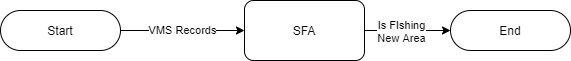
\includegraphics[width=0.8\linewidth]{Chapters/img/Block1-Page-1.png}
\caption{Block Diagram of solution to goal 1.}
\label{fig:block_sfa}
\end{figure}

\subsection{Joined Fishery Analysis} % (fold)
\label{sec:int_jfa}

The proposed solution to objective 2 is the creation of a model that can be used in a system that receives data from various vessels and classifies that data by the type of fishing license. The objective is to understand whether the result of the classification algorithm is compatible or not with the vessel's fishing license.
In this classification problem different methodologies are used, such as,  Decision Trees, Random Forests, Neural Networks and Support Vector Machines algorithms.
In Figure \ref{fig:block_jfa} is presented the solution blocks diagram for the second goal.  We will call this solution \gls{jfa}.

\begin{figure}[h]
\centering
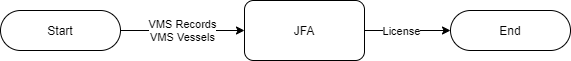
\includegraphics[width=0.8\linewidth]{Chapters/img/Block1-Page-2.png}
\caption{Block Diagram of solution to goal 2.}
\label{fig:block_jfa}
\end{figure}

\section{Thesis Structure} % (fold)
\label{sec:work_structure}
The remainder of this document is organized into six main chapters. Chapter 2 gives an overview of the State of the Art are presented the methods, approaches and tools of the state of the art and their main results and functionality. Reference articles are presented and the main basic methodologies used in each case are explained. 
In Chapter 3 we present two different methodologies to classify the data in real-time, only using the available data by the Blue Box:
\begin{itemize}
\item Using velocity data, to classify if the vessel is fishing;
\item Using location data, to classify if the vessel is in activity in a new area.
\end{itemize}
For the solution the proposed approaches are presented in the form of an algorithm, clearly explaining the input and output parameters. All the actions of the applied techniques are described and presented, so that they can be reproduced by others.
In chapter 4 we presented an approach to answer the second objective: using the data from all the vessels, how to identify fishing activities that are not under the vessel's fishing license. Different data mining methods will be used to derive predictive models. Corresponding results are compared through correct classification performance measures.
Chapter 5 is presented with the results of the validation of the models and methods presented to answer the proposed objectives.
Chapter 6 contains the conclusions obtained during the elaboration of this work.

% section work_structure (end)




